\documentclass[11pt]{article}
\usepackage{amsmath}
%\usepackage{extsizes}
\usepackage{amsmath,amssymb,amsthm}
%\usepackage{omegavn,ocmrvn}
%\usepackage[utf8x]{inputenc}
\usepackage[utf8]{vietnam}

\usepackage{listings}
\lstset{language=Python}          % Set your language (you can change the language for each code-block optionally)
\usepackage[most]{tcolorbox}

\usepackage{longtable}
\usepackage{answers}
\usepackage{graphicx}
\usepackage{array}
\usepackage{pifont}
\usepackage{picinpar}
\usepackage{enumerate}
\usepackage[top=3.0cm, bottom=3.5cm, left=3.5cm, right=2.5cm] {geometry}
\usepackage{hyperref}



\newtheorem{thm}{Theorem}
\newtheorem{definition}{Định nghĩa}
\newtheorem{bt}{Câu}
\newcommand{\RR}{\mathbb R}
\Newassociation{sol}{Solution}{ans}
\newtheorem{ex}{Câu}
\renewcommand{\solutionstyle}[1]{\textbf{ #1}.}
\def\im{\mathrm{im}}

\begin{document}
% \noindent

\begin{tabular*}
	{\linewidth}{c>{\centering\hspace{0pt}} p{.7\textwidth}}
	Trường ĐHKHTN, ĐHQGHN & {\bf Học Kỳ 2 (2021-2022)}
	\tabularnewline
	K64 TTƯD - Thầy Hà Phi & {\bf Bài Tập Giải Tích Số \\ \today}
	% Exercises on pages 239, 240 Cheney/Kincaid are really nice
	\tabularnewline
	\rule{1in}{1pt}  \small  & \rule{2in}{1pt} %(Due date:)
	\tabularnewline
	%  \tabularnewline
	%  &(Đề thi có 1 trang)
\end{tabular*}




\begin{center}
	{\bf Bài Tập Lý Thuyết Điều Khiển Hệ Thống - No. 3 \\
	     Controllability of LTI systems}
\end{center}

\begin{bt}
%a) 
Nhắc lại bài giảng trên lớp.
\begin{tcolorbox}[colback=red!5!white,colframe=green!75!black]
\textbf{Định lý đối ngẫu:} Hãy chứng minh rằng với hệ LTV là C-ctrb với mọi $t_1>t_0$ khi và chỉ khi với mọi nghiệm $z(t)$ của phương trình liên hợp $\dot{z}= - A(t)^Tz$ nà thỏa mãn tính chất trực giao $<z(t),B(t)> = 0$ với mọi $t\in [t_0,\infty)$ khi và chỉ khi $z \equiv 0$.
\end{tcolorbox}
%b) Hãy tự chứng minh/hoặc đọc Chứng minh của Định lý 6.1 (cuốn Chen) về các điều kiện tương đương cho tính chất điều khiển được. 
\end{bt}

\begin{bt}
	Chuyển các hệ điều khiển LTI cấp $n$ sau về hệ điều khiển cấp 1 với biến điều khiển $u$, biến trạng thái $x$ và xét tính điều khiển được của hệ cấp 1 thu được. \\
	a) 
	%
	\begin{equation}
		x^{(n)} + \a_{n-1} x^{(n-1)} + \dots + \a_1 \dot{x} + \a_0 x = u(t) 
	\end{equation}
	%
	b) 
	\begin{equation}
		x^{(n)} + \a_{n-1} x^{(n-1)} + \dots + \a_1 \dot{x} + \a_0 x = 
		u^{(n)} + \b_{n-1} u^{(n-1)} + \dots + \b_1 \dot{u} + \b_0 u \ . 
	\end{equation} 
\end{bt}

\begin{bt}
Các hệ thống sau có điều khiển được hay không? Vì sao? Tìm hàm truyền của các hệ thống đó.\\
\noindent	a) \textbf{Dạng chính tắc điều khiển được (controllability canonical form)}
	%
	\begin{align}
		\dot{x} &= \m{0 & 1 & &  & \\ &  \ddots & \ddots &  & \\ & & \ddots & \ddots &   \\&  &  & 0 & 1 \\ -\a_1 & -\a_2 & \dots & \dots & -\a_{r} } x + \m{0 \\ \vdots \\ \vdots \\ 0 \\ 1} u, \\
		y &= \m{\b_1 &  \dots & \dots & \b_r} x + D u, 
	\end{align}
	%
	trong đó $\a_i$, $\b_i$, $D$ là các hệ số (thực hoặc phức). \\
\noindent	b) \textbf{Dạng chính tắc quan sát được (observability canonical form)}
	%
	\begin{align}
		\dot{x} &= \m{-\a_1 & 1 & &  & \\ \vdots &   & \ddots &  & \\ \vdots & & & \ddots &   \\ -\a_{r-1} &  &  &  & 1 \\ -\a_{r} & 0 & \dots & \dots & 0} x + \m{\b_1 \\  \vdots \\ \vdots \\ \b_{r-1} \\ \b_r} u, \\
		y &= \m{1 &  0 & \dots & \dots & 0} x + D u, 
	\end{align}
	%
	trong đó $\a_i$, $\b_i$, $D$ là các hệ số (thực hoặc phức). 
\end{bt}

\begin{bt} \textbf{Nghiên cứu về tính điều khiển được của 2 hệ thống được mắc nối tiếp/song song với nhau theo các sơ đồ trong Hình \ref{fig:electricalconnection}.} \\
	
	\begin{figure}[!h]
		\centering
		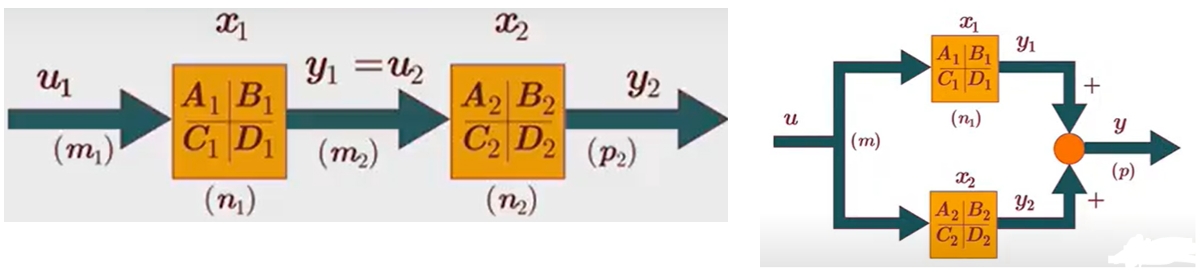
\includegraphics[scale = 0.6]{Figures/Electrical_connection}
		\caption{Mạch nối tiếp (trái) \& Mạch song song (phải)}
		\label{fig:electricalconnection}
	\end{figure}
	
	\noindent Giả sử rằng các hệ con đều là điều khiển được. \\
	a) Chứng minh rằng nếu hệ thống tổng là điều khiển được thì nó không thể có vector riêng trái dạng $w = \m{w_1 & 0} \in \C^{n_1+n_2}$ mà thỏa mãn điều kiện $w^H B= 0$ . \\
	b) Chứng minh hệ thống song song sẽ đánh mất tính điều khiển được khi và chỉ khi $A_1$ và $A_2$ có giá trị riêng chung $\lambda$, và các vector riêng trái $w_1$, $w_2$ tương ứng thỏa mãn
	\begin{align*}
		& w^H_1 B_1 + w^H_2 B_2 = 0, \\
		& w^H_1 A_1 = \lambda w^H_1,   \   w^H_2 A_2 = \lambda w^H_2.
	\end{align*}
\end{bt}

\begin{bt}
	a) Chứng minh rằng đối với hệ LTI 
	%
	\begin{equation}\label{eq1}
		\dot{x} = Ax + Bu, \quad \forall t \geq t_0
	\end{equation}
	%
	thì tính chất điều khiển được là tức thời (instantaneous), tức là nếu nếu hệ là điều khiển được với $t_1 >t_0$ nào đó thì nó cũng điều khiển được với mọi thời điểm $t_2 >t_0$. \\
	\vskip .2cm
	\noindent b) Xét hệ thống điều khiển LTI có dạng \eqref{eq1}. Trong một số ứng dụng thực tế, ví dụ như các hệ cơ học, nhiều khi người ta không quan tâm đến toàn bộ trạng thái $x(t)$ mà chỉ 1 phần của nó, tức là phần $Lx$, trong đó $L$ là một ma trận. Khi đó hệ được gọi là điều khiển được 1 phần (\textbf{partial controllable}) như trong định nghĩa sau.
	
	\begin{tcolorbox}[colback=red!5!white,colframe=green!75!black]
		\begin{definition}
			Hệ LTI được gọi là L-ctrb, trong đó $L \in \R^{\ell,n}$ là một ma trận với cỡ $\ell \times n$ có đủ hạng dòng, nếu như với mọi trạng thái $x_1 \in \R^n$ tồn tại một hàm đầu vào $u$ và một thời điểm $t_1 >t_0$ sao cho $Lx(t_1;t_0,x_0,u) = Lx_1$.  
		\end{definition} 
	\end{tcolorbox}
	
	Hãy xây dựng và chứng minh điều kiện đủ cho tính chất L-điều khiển được thông qua các điều kiện hạng Kalman (phần c), hạng Hautus (phần d) và Gramian điều khiển. 
\end{bt}


\end{document}

\begin{bt}
	Mệnh đề sau có luôn luôn đúng không?
	%
	\[
	\rank \m{B & A B & \dots & A^{n-1}B} = \rank \m{AB & A^2 B & \dots & A^{n} B} \ .
	\]
	% 
	Nếu không, nó sẽ đúng với điều kiện nào?
\end{bt}

\begin{bt}
	Đối với hệ LTI, hãy chứng tỏ rằng $(A, B)$ là điều khiển được khi và chỉ khi $(-A, B)$ là điều khiển được. Điều này có đúng với các hệ thống LTV không?
\end{bt}   

\begin{bt}
	Hãy xét tính điều khiển được của các hệ điều khiển sau
	%
	\begin{equation}
		\dot{x} = \m{0 & 1 & 0 \\ 0 & 0 & 1 \\ 1 & -3 & -3} x + \m{0 \\ 0 \\ 1} u, \quad
		y = \m{1 & 2 & 1} x. 
	\end{equation}
\end{bt}
%
